\subsection{Two-Stage Newsvendor Model}

Let us consider a case where we have a two-period planning horizon, rather than one as we had for the newsvendor problem. Here, at the beginning of each period, we  first observe the current inventory level, and then we decide upon the order quantity. Thus, this case  becomes an extension of the newsvendor model, because now we have an extra ordering moment in the middle of the day. 

For convenience, we use the same notation that we used for the single-period newsvendor model. However, we add a period index to the buying and selling prices as well as the demand distribution (i.e. $c_n$, $p_n$, and $g_n(\cdot)$ where $n\in\{1,2\}$), as these can be different in the morning and in the afternoon.

\begin{question}
Suppose the afternoon demand is $D_2\in \{0,1,2\}$ and $g_2(0)=g_2(1)=g_2(2)=1/3$.  Consider  three cases: at the end of the morning you have  0, 1, and 2 items in stock. What would be the best number of items $Q_2$ to order at start of the second period (the afternoon) for each of these cases? (It is perhaps the easiest to use Eq.~\eqref{eq:1}.)

\begin{solution}
	It is obvious that we do not need more than 2 items in the afternoon, because the demand $D_2\leq 2$ always.
	
	\begin{itemize}
	
	\item In the first case (no stock at the end of the morning), our options for $Q_2$ are ordering 0, 1, or 2 items. Take $Q_2=0$ first. Then we see that 
    \begin{equation*}
P(Q_2=0) = (p -c)Q_2  + (s-p)\E{(Q_2-D_2)^+} = (p -c) 0   + (s-p)\E{(0-D_2)^+} = 0.
\end{equation*}
The profit of the choice $Q_2=1$ is 
    \begin{equation*}
P(1) = (p -c)1  + (s-p)\E{(1-D_2)^+}. 
\end{equation*}
Now
\begin{equation*}
  \begin{split}
\E{(1-D_2)^+}
&=(1-0)^+\P{D_2=0} + (1-1)^+\P{D_s=1} + (1-2)^+ \P{D_2=2} \\
&= 1 \P{D_2=0} = 1\cdot 1/3 = 1/3.
  \end{split}
\end{equation*}
Therefore
    \begin{equation*}
P(1) = (p -c)1  + (s-p) 1/3.
  \end{equation*}
Finally, the profit for choice $Q_2=2$ is 
    \begin{equation*}
P(2) = (p -c)2  + (s-p)\E{(2-D_2)^+} = (p-c)2 + (s-p).
\end{equation*}
since
\begin{equation*}
  \begin{split}
\E{(2-D_2)^+}
&=(2-0)^+\P{D_2=0} + (2-1)^+\P{D_s=1} + (2-2)^+ \P{D_2=2} \\
&= 2\cdot 1/3 + \cdot 1/3 = 1.
  \end{split}
\end{equation*}

\item When the inventory at the end of the morning is $1$,  our options are ordering $Q_2=0$ or $Q_2=1$ items. Now if we order $Q_2$, the inventory at the start of the second period is $1+Q_2$. Thefore, the profit function takes the form
    \begin{equation*}
P(Q_2) = (p -c)Q_2  + (s-p)\E{(Q_2+1-D_2)^+}. 
\end{equation*}
Hence, 
    \begin{equation*}
P(0) = (s-p)\E{(1-D_2)^+},
\end{equation*}
and we already computed this expectation above. Also
    \begin{equation*}
P(1) = (p -c)1  + (s-p)\E{(2-D_2)^+}. 
\end{equation*}
  
  \item In the third case, i.e., starting with $2$ items in stock, 
    \begin{equation*}
P(Q_2) = (p -c)Q_2  + (s-p)\E{(Q_2+2-D_2)^+}. 
\end{equation*}
In this case, the  decision is easy as we already have the maximum amount of items that we might possibly need. So the only reasonable choice is $Q_2=0$.  Its profit is 
    \begin{equation*}
P(0) = (s-p)\E{(2-D_2)^+}. 
\end{equation*}
\end{itemize}
\end{solution}
\end{question}

\begin{question}
Explain why the decision on how many items to make in the afternoon depends on the number of items that is left from the morning. 

\begin{solution}
The items that are left from the morning contributes to the profit in the afternoon. That is due to two reasons: (1) We don't have to pay in the afternoon to acquire what we already have in stock as leftovers from the morning (in other words, there is no purchasing cost for leftovers), and (2) if there are more leftovers  than what is actually needed, it is optimal  to not make new items. 
\end{solution}
\end{question}


\begin{question}
Suppose the morning demand is $D_1\in \{0,1,2\}$ and $g_1(0)=g_1(1)=1/4$, $g_1(2)=1/2$; and the afternoon demand is $D_2\in \{0,1\}$ and $g_2(0)=g_2(1)=1/2$. It is not possible to backlog demands, that is,  demands not satisfied in the morning are lost. Also, we have that $c_1=10$, $c_2=12$, $p_1=p_2=20$, and $s=5$. Now, assume that we make 2 items in the morning. What is the expected total profit in the morning and in the afternoon?
\begin{solution}
TBD.

%Let us start with the afternoon. The following are the expected profits (disregarding the purchasing costs) in the afternoon, if the inventory level after making new items is 0, 1, 2, respectively:
%\begin{align*}
%    \text{(start with $0$ item)} \quad  & 0 & = 0 \\
%    \text{(start with $1$ item)} \quad  & p_{s2} \cdot 1/2 + p_e \cdot 1/2 & = 12.5 \\
% 	\text{(start with $2$ items)} \quad  & p_{s2} \cdot 1/2 + p_e \cdot 3/2 & = 17.5
%\end{align*}  
%
%If we make 2 items in the morning, then at the end of the morning 
%\begin{itemize}
%\item with probability $\P(X_1=2)=1/2$ we sell 2 items, make a profit of $-p_{b1} 2 + p_{s1} 2$, and end up with $2-2=0$ items
%\item with probability $\P(X_1=1)=1/4$ we sell 1 item, make a profit of $-p_{b1} 2 + p_{s1} 2$
%
%\end{itemize}
%
%
%
%
%,  we end up with $2-1=1$ items, and with probability $\P(X_1=0)=1/4$ we end up with $2-0=0$ items. 
%
%
%the probability of ending up with 0, 1, 2 items at the end of the morning are: $\P(2-X_1=0)=\P(2-X_1=0)$

\end{solution}

\end{question}

\begin{question}
Let $U(A)$ be a function that returns the expected profit in the afternoon, given that the inventory level after making new items is $A$. What are the general terms that make up this function?
   \begin{solution}
     TBD.
   \end{solution}
\end{question}

\begin{question}
How can one make use of $U(A)$ when deciding the number of items $Q_2$ to make in the afternoon?
   \begin{solution}
     TBD.
   \end{solution}
\end{question}

\begin{question}
Let $V(I)$ be a function that returns the expected profit in the afternoon, given that the inventory level after before making new items is $I$. What are the general terms that make up this function?
   \begin{solution}
     TBD.
   \end{solution}
\end{question}

\begin{question}
Write $U(A)$ and $V(I)$ in terms of probabilities $g_2(i)=\P(X_2=i)$
   \begin{solution}
     TBD.
   \end{solution}
\end{question}

\begin{question}
Let $Z(Q_1)$ be a function that returns the expected profit over the whole day given $Q_1$ items are produced in the morning is $I$. What are the general terms that make up this function?
   \begin{solution}
     TBD.
   \end{solution}
\end{question}

\begin{question}
Write $Z(Q)$ in terms of probabilities $g_1(i)=\P(X_1=i)$
   \begin{solution}
     TBD.
   \end{solution}
\end{question}

\begin{question}
We have so far assumed that the sequence of events over the day were as follows: (1) decide $Q_1$, (2) observe $X_1$, (3) decide $Q_2$, (4) observe $X_2$. How would we set order quantities if the sequence of events were as follows (1) decide $Q_1$ and $Q_2$, (2) observe $X_1$, (3) observe $X_2$.
   \begin{solution}
     TBD.
   \end{solution}
\end{question}

\begin{question}
What is the financial value of having an second ordering moment in the middle of the day, after observing the demand in the morning?
   \begin{solution}
     TBD.
   \end{solution}
\end{question}

\begin{question}
We have thus far considered profit functions $U(A)$, $V(I)$, and $Z(Q_1)$. Can you devise cost functions for the same two-period newsvendor problem?
   \begin{solution}
     TBD.
   \end{solution}
\end{question}

\begin{question}
We have thus far considered profit functions $U(A)$, $V(I)$, and $Z(Q_1)$. Can you devise cost functions for the same two-period newsvendor problem?
   \begin{solution}
     TBD.
   \end{solution}
\end{question}

\begin{question} A Case to  Get rich in \st{one day} two days. 

  \begin{itemize}
  \item You plan to sell Napoleons tomorrow and the next day just outside of the Duisenberg building.
  \item How much money can you make? 
  \item How many Napoleons would you order for each day if you can sell left Napoleons from the first day in the second one?
  \end{itemize}

   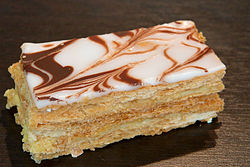
\includegraphics[scale = 1.0]{figures/mille-feuille}
   %\includegraphics[scale = 1.0]{250px-Mille-feuille_20100916}

%   \begin{solution}
%Here are the steps.
%  \begin{itemize}
%  \item Let's first assume that demand is normally distributed. Then
%    we know from FP that $Q$ should be such that
%    $G(Q) = c_s/(c_s+c_o)$.
%  \item We make some assumptions about the prices. Take $p_s=0.75$,
%    $p_b = 0.25$. $p_e=0$. Hence, $c_o = 0.25$, and $c_s = 0.5$.
%  \item Thus, the critical fraction is $c_s/(c_s+c_o)=0.5/0.75 = 2/3$.
%  \item Now compute $z$ with $\Phi(z)=2/3.$. Hence $z=0.43$.
%  \item We also need some idea about the demand. How to get this?
%  \item For Napoleons, we don't have yesterday's demand \ldots
%  \item Can we use demand data of similar products?  I don't know what
%    data to use. I have never tried to sell napoleons.
%  \item Can we ask our sales force?  no. We don't have a sales force. 
%  \item Last resort: make an educated guess; use powers of ten
%    trick. Under this price model, I expect to sell more 1 napoleon,
%    also more than 10, 100 might be, 1000 is too much. So, take
%    $\mu=100$ as an estimate. Since I am not sure, $\sigma=30$ seems
%    reasonable.
%  \item If $\mu = 100$ and $\sigma = 30$, then $Q=0.43\sigma + \mu \approx 112$.
%  \item Finally, what is the profit $Z(Q)$?
%\item With the above formulas you can compute $Z(Q)$,  but let's use handwaving for a quick estimate. 
%\item Note that $\min\{Q, X\} \leq X$, hence
%  $\E \min\{X, Q\} \leq \E X= \mu$. If $\E \min\{X, Q\}\approx 95$,
%  then $Z(112) \approx 95r - 100 c = 95\cdot 0.75 - 100 \cdot 0.25$.
%  Since $95f\approx100$, use this to simplify yet more:
%  $Z(112) \approx 100(0.75-0.25) = 50$ Euro.
%\item There are easier ways to make money!
%  \end{itemize}
%\end{solution}
\end{question}

\begin{question}
Can you generalize the two-period newsvendor case to an arbitrary number of periods?
   \begin{solution}
     TBD.
   \end{solution}
\end{question}

\begin{question}
Can you generalize the two-period newsvendor case to an infinite number of periods?
   \begin{solution}
     TBD.
   \end{solution}
\end{question}


%%% Local Variables:
%%% mode: latex
%%% TeX-master: t
%%% End:
